\documentclass[aspectratio=169,10pt]{beamer}
\usetheme{Madrid}
\usecolortheme{seahorse}
\usefonttheme{professionalfonts}

\setbeamertemplate{footline}[frame number]
\setbeamertemplate{navigation symbols}{}

\usepackage{amsmath,amssymb,mathtools}
\usepackage{graphicx}
\usepackage{booktabs}
\usepackage{listings}
\usepackage{xcolor}
\usepackage{tikz}
\usetikzlibrary{arrows.meta,positioning}

\graphicspath{{figures/}}

\lstset{
  basicstyle=\ttfamily\scriptsize,
  numbers=left,
  numberstyle=\tiny,
  frame=single,
  backgroundcolor=\color{gray!7},
  commentstyle=\color{green!50!black}\itshape,
  keywordstyle=\color{blue!70!black}\bfseries,
  stringstyle=\color{orange!70!black},
  showstringspaces=false,
  breaklines=true,
  language=Python,
}

\newcommand{\R}{\mathbb{R}}
\newcommand{\N}{\mathbb{N}}
\newcommand{\E}{\mathbb{E}}
\newcommand{\Pb}{\mathbb{P}}
\newcommand{\Qb}{\mathbb{Q}}
\newcommand{\calK}{\mathcal{K}}
\newcommand{\calP}{\mathcal{P}}
\newcommand{\calN}{\mathcal{N}}
\newcommand{\calD}{\mathcal{D}}

\title[E-Values -- Ch.10]{Hypothesis Testing with E-Values}
\subtitle{Chapter 10: Approximate and Asymptotic E-Values}
\author{Based on Ramdas \& Wang}
\date{}

\begin{document}

\begin{frame}
  \titlepage
\end{frame}

\begin{frame}[allowframebreaks]{Outline}
  \tableofcontents
\end{frame}

% ============================================================
\section{Setup and notation}
% ============================================================

\begin{frame}[allowframebreaks]{Why bother with approximate or asymptotic e-values?}
  \textbf{The problem.} So far, an e-variable $E$ for a null $\Pb$ had to satisfy $\E^{\Pb}[E] \leq 1$ \emph{exactly}, for every $\Pb$ in the null, no matter the sample size. That is a strong requirement. In practice:
  \begin{itemize}
    \item We often only know how to construct an e-value that satisfies $\E^{\Pb}[E]\leq 1$ up to some small, known slack -- e.g.\ because of a plug-in estimate, a truncation, or a numerical approximation.
    \item Even more commonly, we only know that a statistic \emph{becomes} valid as the sample size $n \to \infty$ -- this is exactly the situation whenever we invoke the Central Limit Theorem (CLT) to justify a $Z$-test or $t$-test.
  \end{itemize}

  \vspace{0.2cm}
  \textbf{This chapter's job:} make these two relaxations -- \emph{approximate} (Section 10.1) and \emph{asymptotic} (Section 10.2) -- mathematically precise, show they compose well with calibration (converting p-values $\leftrightarrow$ e-values), give the single most important construction (the CLT-based e-value, Section 10.3), and extend everything to \emph{multiple} testing (Section 10.4).

  \framebreak

  \textbf{Roadmap of the chapter.}
  \begin{enumerate}
    \item \textbf{10.1} Approximate p-/e-values: a \emph{fixed}, known error budget $(\varepsilon,\delta)$ at any single sample size.
    \item \textbf{10.2} Asymptotic p-/e-values: a \emph{sequence} of approximate p-/e-values indexed by $n$, whose error budget $(\varepsilon_n,\delta_n) \to (0,0)$ as $n\to\infty$.
    \item \textbf{10.3} The single most useful asymptotic e-value in practice: built from the CLT, for testing a population mean when the variance is unknown.
    \item \textbf{10.4} The same three ideas (exact / approximate / asymptotic), but now for \emph{compound} e-values used in multiple testing and FDR control (Chapter 9).
  \end{enumerate}
\end{frame}

\begin{frame}[allowframebreaks]{Notation you'll need}
  \textbf{Intuition first.} An \emph{exact} e-value never lies (in expectation) -- but exact constructions are not always available. An \emph{approximate} e-value lies a little, but by a known, bounded amount -- you can always account for the slack. An \emph{asymptotic} e-value's lie shrinks to zero only as $n\to\infty$ -- at any \emph{fixed}, finite $n$ you have no numerical guarantee at all, only the promise that the guarantee improves as more data arrives.

  \begin{block}{Exact vs.\ approximate vs.\ asymptotic e-values}
    \begin{tabular}{@{}p{2.1cm}p{4.6cm}p{4.6cm}@{}}
      \toprule
      \textbf{Type} & \textbf{Defining condition} & \textbf{What you actually get} \\
      \midrule
      Exact & $\E^{\Pb}[E] \leq 1$ for every $\Pb$ in the null, at the sample size you have. & A hard guarantee, right now, with zero slack. \\[0.15cm]
      Approximate $(\varepsilon,\delta)$ & $\E^{\Pb}[E \wedge t] \leq 1+\varepsilon+\delta t$ for all $t\in\R_+$, at the sample size you have. & A guarantee with a \emph{known, bounded} error: $\varepsilon\geq0$ is a multiplicative slack, $\delta\in[0,1]$ is a probability-of-failure slack. Still holds at any fixed $n$. \\[0.15cm]
      Asymptotic & A \emph{sequence} $(E^{(n)})_n$ that is $(\varepsilon_n,\delta_n)$-approximate with $\varepsilon_n(\Pb)\to0,\ \delta_n(\Pb)\to0$ as $n\to\infty$. & \emph{No} numerical guarantee at any single finite $n$ -- only that the error vanishes in the limit $n\to\infty$. \\
      \bottomrule
    \end{tabular}
  \end{block}
  Here $E\wedge t := \min(E,t)$; capping $E$ at a threshold $t$ before taking expectations is what makes the definition work even for $E$ that can be infinite (recall $E$ is $[0,\infty]$-valued).

  \framebreak

  \textbf{Two different kinds of error, $\varepsilon$ and $\delta$.} Definition 10.1 in the book distinguishes two ways an object can fail to be a genuine p-/e-variable:
  \begin{block}{$\varepsilon$: a multiplicative value-error}
    Measures how far the \emph{value} of the random variable is from a genuine p-/e-variable. Example: if $P \sim \mathrm{U}(0,1)$ is a genuine p-variable, then $(1+\varepsilon)P$ is ``$\varepsilon$-away'' -- every realization is inflated by the same known factor.
  \end{block}
  \begin{block}{$\delta$: a probability-of-failure error}
    Measures \emph{how often} (in probability) the object deviates from being a genuine p-/e-variable. Example: if $P \sim \mathrm{U}[0,1]$ and $A$ is an event with $\Pb(A) = 1-\delta$, then $P\mathbb{1}_A$ is ``$\delta$-away'' -- it behaves perfectly on $A$, and is simply set to $0$ (an automatic rejection) with probability $\delta$.
  \end{block}
  The two error types are asymmetric: $\delta$ is the more lenient/forgiving of the two (Proposition 10.5 below makes this precise).

  \framebreak

  \textbf{CLT recap (the tool that powers all of Section 10.3).} Let $X^1,\dots,X^n$ be i.i.d.\ real random variables with $\E[X^i]=\mu$ and $\mathrm{var}(X^i)=\sigma^2\in(0,\infty)$. Write the sample mean $\bar X^{(n)} = \frac1n\sum_{i=1}^n X^i$.
  \begin{block}{Central Limit Theorem}
    \[
      \sqrt n \, \frac{\bar X^{(n)} - \mu}{\sigma} \ \xrightarrow{\ d\ }\ \mathrm{N}(0,1) \qquad \text{as } n \to \infty,
    \]
    i.e.\ for large $n$, $\bar X^{(n)}$ is \emph{approximately} Gaussian with mean $\mu$ and variance $\sigma^2/n$: $\bar X^{(n)} \approx \mathrm{N}(\mu, \sigma^2/n)$. The concrete variance formula $\mathrm{var}(\bar X^{(n)}) = \sigma^2/n$ is exactly why more data ($n\to\infty$) shrinks the spread of $\bar X^{(n)}$ around $\mu$ to zero.
  \end{block}
  This is an \emph{asymptotic} statement: it says nothing exact about any fixed $n$, only that the approximation error vanishes as $n\to\infty$ -- exactly the spirit of ``asymptotic'' e-values we formalize next.
\end{frame}

% ============================================================
\section{10.1 Approximate p-values and e-values}
% ============================================================

\begin{frame}{10.1 Intuition: allowing a known amount of slack}
  \textbf{Why not require exactness always?} Sometimes we can prove a statistic is \emph{almost} a valid p-/e-variable, with an error we can bound explicitly -- e.g.\ from a plug-in variance estimate, a discretization, or a truncation used for computational reasons. Definition 10.1 packages this ``almost valid, with a known bound on how far off'' idea into two tuning knobs, $\varepsilon$ (value-error) and $\delta$ (probability-error), that can be set to $0$ to recover the exact definitions.
\end{frame}

\begin{frame}{Definition 10.1: approximate p-variables and e-variables}
  Fix the null $\calP$ and two functions $\varepsilon:\calP\to\R_+$, $\delta:\calP\to[0,1]$; write $\varepsilon_\Pb=\varepsilon(\Pb)$, $\delta_\Pb=\delta(\Pb)$.
  \begin{block}{$(\varepsilon,\delta)$-approximate p-variable}
    An $\R_+$-valued random variable $P$ is $(\varepsilon,\delta)$-\emph{approximate} for $\calP$ if
    \[
      \Pb(P\leq t) \leq (1+\varepsilon_\Pb)\,t + \delta_\Pb \qquad \text{for all } t\in(0,1),\ \Pb\in\calP.
    \]
    Here $t$ ranges over candidate significance thresholds; the right side inflates the ideal bound $t$ by a multiplicative factor $1+\varepsilon_\Pb$ and an additive slack $\delta_\Pb$.
  \end{block}
  \begin{block}{$(\varepsilon,\delta)$-approximate e-variable}
    A $[0,\infty]$-valued random variable $E$ is $(\varepsilon,\delta)$-\emph{approximate} for $\calP$ if
    \[
      \E^{\Pb}[E\wedge t] \leq 1+\varepsilon_\Pb+\delta_\Pb t \qquad \text{for all } t\in\R_+,\ \Pb\in\calP.
    \]
  \end{block}
  Setting $\varepsilon\equiv0,\delta\equiv0$ recovers ordinary p-/e-variables exactly. If $\delta_\Pb=1$, the definition is vacuous (no constraint at all) -- so $\delta$ close to $1$ buys almost nothing.
\end{frame}

\begin{frame}{Proposition 10.2: an equivalent, more intuitive picture}
  \textbf{Intuition.} Rather than an abstract inequality, you can picture $(\varepsilon,\delta)$-approximation concretely: there is a ``good'' event $A$, of probability at least $1-\delta_\Pb$, on which the object behaves like an honest $(\varepsilon_\Pb,0)$-approximate p-/e-variable; outside $A$ (probability $\leq \delta_\Pb$), anything at all can happen.
  \begin{block}{Proposition 10.2}
    For every $\Pb\in\calP$ there exists an event $A$ such that:
    \[
      \text{(p-variable)}\quad \Pb(P\leq t, A) \leq (1+\varepsilon_\Pb)t \ \ \forall t\in(0,1), \qquad \Pb(A)\geq 1-\delta_\Pb;
    \]
    \[
      \text{(e-variable)}\quad \E^{\Pb}[E\mathbb{1}_A] \leq 1+\varepsilon_\Pb, \qquad \Pb(A)\geq 1-\delta_\Pb.
    \]
    This event-based statement always \emph{implies} the Definition 10.1 inequality; the two are fully \emph{equivalent} whenever every $\Pb\in\calP$ is atomless (so we can construct $A$ exactly at the right probability level).
  \end{block}
\end{frame}

\begin{frame}{Calibration still works: Theorem 10.3 and Proposition 10.5}
  \begin{block}{Theorem 10.3 (calibration is preserved)}
    Using any (p-to-e or e-to-p) calibrator, calibrating an $(\varepsilon,\delta)$-approximate p-variable yields an $(\varepsilon,\delta)$-approximate e-variable, and vice versa.
  \end{block}
  This means all the calibration machinery from Chapter 2 (e.g.\ $f(x)=1/\sqrt x$ or any decreasing density calibrator) carries over verbatim to the approximate setting -- you do not need new calibrators.

  \vspace{0.2cm}
  \begin{block}{Proposition 10.5 ($\delta$ is more forgiving than $\varepsilon$)}
    Let $\delta' = (\varepsilon+\delta)/(1+\varepsilon)$. Any $(\varepsilon,\delta)$-approximate p-variable (or e-variable) for $\calP$ is automatically also a $(0,\delta')$-approximate p-variable (or e-variable) for $\calP$, with $\delta' $ strictly smaller than $\varepsilon+\delta$ whenever $\varepsilon>0$.
  \end{block}
  Interpretation: you can always trade a bit of multiplicative slack $\varepsilon$ for a (smaller) increase in probability slack $\delta'$ -- so $\delta$-type approximation is the more general, more lenient notion. This asymmetry is why Section 10.2 below builds two \emph{different} flavors of ``asymptotic'' out of $\varepsilon_n\to0$ alone versus $\varepsilon_n,\delta_n\to0$ jointly.
\end{frame}

\begin{frame}[fragile]{Python: 10.1 -- an $(\varepsilon,\delta)$-approximate p-value in action}
  \begin{lstlisting}
import numpy as np
rng = np.random.default_rng(0)

N = 200_000
U = rng.uniform(0, 1, size=N)          # genuine p-variable: U ~ Unif(0,1)

eps, delta = 0.10, 0.05                 # known error budget

# Construct an (eps, delta)-approximate p-variable "by hand":
# (a) inflate values by (1+eps) on a "good" event A of probability 1-delta,
# (b) force P = 1 (never falsely reject) on the complement of A.
A = rng.uniform(0, 1, size=N) <= (1 - delta)
P_tilde = np.where(A, (1 + eps) * U, 1.0)

t = 0.05                                # a candidate significance level
lhs = np.mean(P_tilde <= t)             # empirical P(P_tilde <= t)
rhs = (1 + eps) * t + delta             # Definition 10.1 bound
print(f"P(P_tilde <= {t}) = {lhs:.4f}   vs.  (1+eps)t + delta = {rhs:.4f}")
# lhs should stay safely below rhs -- the approximate p-value bound holds
  \end{lstlisting}
\end{frame}

\begin{frame}{Figure: exact vs.\ $(\varepsilon,0)$-approximate e-value}
  \centering
  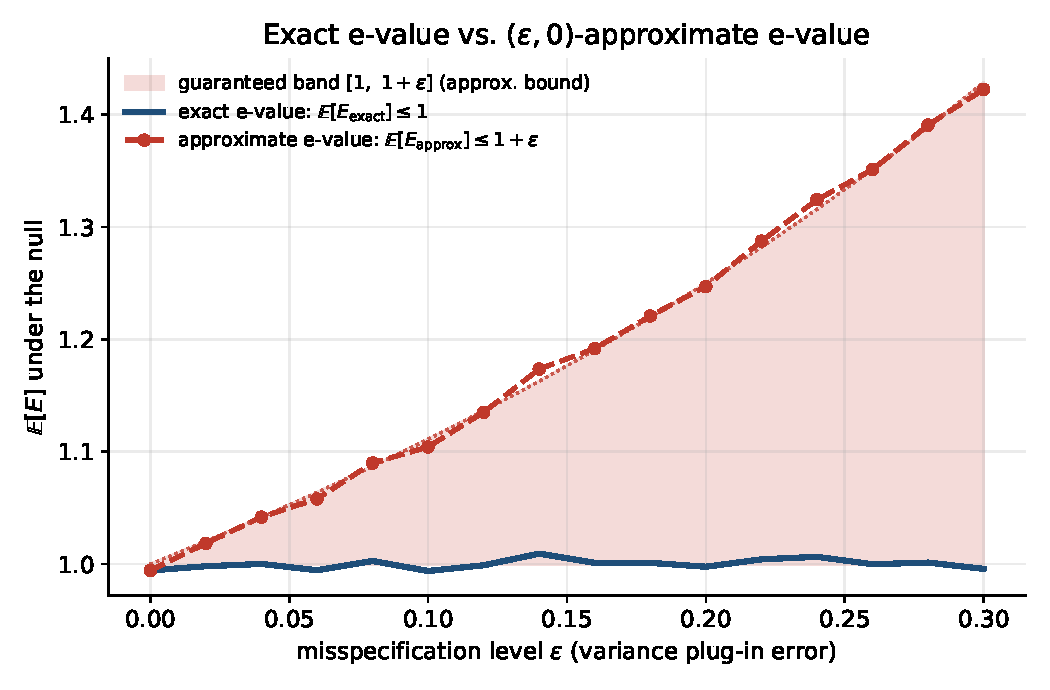
\includegraphics[width=0.72\textwidth]{fig_exact_vs_approximate.pdf}

  \small Null population $\mathrm{N}(0,1)$, testing $\Pb_\sigma=\{\Pb: \E[X]=0,\ \mathrm{var}(X)\leq\sigma^2\}$ (Example 10.12). The exact e-value $E_{\mathrm{exact}}=X^2/\sigma_0^2$ has $\E[E_{\mathrm{exact}}]\leq1$ for every misspecification level $\varepsilon$ (flat blue line). An approximate e-value built from a variance plug-in with a known relative error $\varepsilon$ has $\E[E_{\mathrm{approx}}]\leq 1+\varepsilon$ (red curve, shaded band $[1,1+\varepsilon]$) -- the simulated curve tracks the theoretical bound $1/(1-\varepsilon)\approx1+\varepsilon$ closely.
\end{frame}

% ============================================================
\section{10.2 Asymptotic p-values and e-values}
% ============================================================

\begin{frame}{10.2 Intuition: an entire sequence, with vanishing error}
  \textbf{The idea.} We now observe growing datasets $X^{(1)}, X^{(2)}, \dots$ and compute a statistic $P^{(n)}$ or $E^{(n)}$ from each. Rather than requiring $(\varepsilon,\delta)$-approximation with a \emph{fixed}, known $(\varepsilon,\delta)$ at every $n$, we only ask that \emph{some} sequence $(\varepsilon_n,\delta_n)\to(0,0)$ works -- we do not even need to know the rate of convergence, or the value of $(\varepsilon_n,\delta_n)$ at any particular $n$. This is strictly weaker than approximate validity at each fixed $n$, and it is exactly the guarantee that CLT-based constructions provide.
\end{frame}

\begin{frame}{Definition 10.6: four flavors of ``asymptotic''}
  \begin{block}{Asymptotic e-variables}
    $(E^{(n)})_{n\in\N}$ is a sequence of \emph{asymptotic} e-variables for $\calP$ if $E^{(n)}$ is $(\varepsilon_n,\delta_n)$-approximate for some $(\varepsilon_n,\delta_n)$ with, for each $\Pb\in\calP$: $\lim_n \varepsilon_n(\Pb) = \lim_n \delta_n(\Pb) = 0$.
  \end{block}
  \begin{tabular}{@{}p{3.4cm}p{8.8cm}@{}}
    \toprule
    \textbf{Flavor} & \textbf{Extra requirement beyond ``asymptotic''} \\
    \midrule
    Strongly asymptotic & $\delta_n(\Pb)=0$ for $n$ large enough (not just $\to0$) -- the probability-error disappears completely, eventually. \\
    Uniformly asymptotic & $\sup_{\Pb\in\calP}\varepsilon_n(\Pb)\to0$ and $\sup_{\Pb\in\calP}\delta_n(\Pb)\to0$ -- convergence rate does not depend on which null $\Pb$ is true. \\
    Uniformly strongly asymptotic & Both of the above simultaneously. \\
    \bottomrule
  \end{tabular}
  (Uniformly, strongly) asymptotic p-variables are defined analogously, replacing the e-variable inequality with the p-variable one. If $\calP$ is finite, ``asymptotic'' automatically upgrades to ``uniformly asymptotic.''
\end{frame}

\begin{frame}[allowframebreaks]{Proposition 10.7: useful equivalent characterizations}
  \textbf{Intuition first.} Part (i) is the workhorse: if a sequence of statistics converges \emph{in distribution} to a genuine p-/e-variable, it is automatically an asymptotic p-/e-variable -- this is exactly how the CLT will be used in Section 10.3. Parts (ii)--(iv) restate the definitions in terms of expectations/probabilities, which are often easier to verify directly.
  \begin{block}{Proposition 10.7}
    \begin{enumerate}
      \item If $(P^{(n)})$ (resp.\ $(E^{(n)})$) converges in distribution under every $\Pb\in\calP$ to a genuine p-variable (resp.\ e-variable), it is a sequence of asymptotic p-variables (resp.\ e-variables).
      \item $(E^{(n)})$ is uniformly strongly asymptotic iff $\displaystyle \limsup_n \sup_{\Pb\in\calP} \E^{\Pb}[E^{(n)}] \leq 1$; it is strongly asymptotic iff $\limsup_n \E^{\Pb}[E^{(n)}]\leq1$ for every fixed $\Pb$.
      \item If a sequence of asymptotic e-variables is uniformly integrable (for each $\Pb$), it is strongly asymptotic.
      \item $(P^{(n)})$ is uniformly asymptotic iff $\limsup_n \sup_{\Pb\in\calP}\Pb(P^{(n)}\leq t)\leq t$ for all $t\in(0,1)$.
    \end{enumerate}
  \end{block}

  \framebreak

  \textbf{Why this matters in practice.} Constructions based on convergence in distribution (part (i)) are ubiquitous: Z-tests and t-tests rely on $Z^{(n)} \to \mathrm{N}(0,1)$; likelihood-ratio and $\chi^2$-tests rely on $Z^{(n)} \to \chi^2_\nu$. Whenever $\E[h(Z)]\leq1$ for the limiting law $Z$ and $h$ is increasing/decreasing/upper semicontinuous, Proposition 10.9 (below) turns this convergence directly into a sequence of asymptotic e-variables $E^{(n)}=h(Z^{(n)})$ -- no further work needed. Part (iii) tells us when we get the \emph{stronger} ``strongly asymptotic'' flavor for free: whenever the sequence is uniformly integrable, which is often checkable via a uniform moment bound (as we do for Theorem 10.11 below).

  \begin{block}{Proposition 10.8 (calibration, again)}
    Calibrating a sequence of (uniformly, strongly) asymptotic p-variables -- applying a possibly different calibrator to each element -- yields a sequence of (uniformly, strongly) asymptotic e-variables, and vice versa.
  \end{block}
\end{frame}

\begin{frame}{Proposition 10.9: the general convergence-in-distribution recipe}
  \begin{block}{Proposition 10.9}
    Suppose a statistic $Z^{(n)} \to Z$ in distribution under every $\Pb\in\calP$, where $Z$ has a continuous CDF $F$.
    \begin{enumerate}
      \item $P^{(n)} = F(Z^{(n)})$ or $1-F(Z^{(n)})$ defines a sequence of asymptotic p-variables.
      \item If $h:\R\to[0,\infty)$ is increasing, decreasing, or upper semicontinuous with $\E[h(Z)]\leq1$, then $E^{(n)}=h(Z^{(n)})$ defines a sequence of asymptotic e-variables; if $h$ is also bounded, the sequence is \emph{strongly} asymptotic.
    \end{enumerate}
  \end{block}
  \textbf{Three limiting laws that show up constantly:}
  \begin{itemize}
    \item $Z\sim\mathrm{N}(0,1)$ -- from the CLT (Section 10.3's construction).
    \item $Z\sim|\mathrm{N}(0,1)|$, the folded normal (distribution of $|X|$, $X\sim\mathrm{N}(0,1)$) -- for two-sided tests.
    \item $Z\sim\chi^2_\nu$ -- for likelihood-ratio or chi-square tests.
  \end{itemize}
  This single proposition is the engine behind essentially every classical large-sample test being reinterpreted as producing an asymptotic e-value, not just an asymptotic p-value.
\end{frame}

% ============================================================
\section{10.3 An asymptotic e-value via the central limit theorem}
% ============================================================

\begin{frame}{10.3 Intuition: turning the $Z$-test into an e-value}
  \textbf{The classical picture.} Every introductory statistics course teaches: to test $H_0: \E[X]=0$ with unknown variance, compute $Z^{(n)} = \sqrt n \bar X^{(n)}/S^{(n)}$, and by the CLT this is approximately $\mathrm{N}(0,1)$ under $H_0$ for large $n$ -- giving an (asymptotic) $p$-value.

  \vspace{0.2cm}
  \textbf{The new idea in this section.} Instead of stopping at a p-value, we exploit the \emph{exact} moment generating function identity of the standard normal, $\E[\exp(\lambda Z - \lambda^2/2)] = 1$ for $Z\sim\mathrm{N}(0,1)$, to build an e-value directly out of $Z^{(n)}$. Because $Z^{(n)}$ is only \emph{approximately} Gaussian at finite $n$, the resulting e-value is only \emph{asymptotically} valid -- but this is often the \emph{only} e-value construction available for this null (Theorem 10.11's remark), since no exact, nonasymptotic e-variable is known for testing a mean with completely unknown, unbounded variance.
\end{frame}

\begin{frame}{Step-by-step derivation of the CLT-based e-value}
  \textbf{Setup.} Observe $X^{(n)}=(X^1,\dots,X^n)$, i.i.d.\ $\sim\Pb$, testing $\calP=\{\Pb: \E^{\Pb}[X^i]=0,\ \mathrm{var}^{\Pb}(X^i)\in(0,\infty)\}$ (mean zero, unknown finite variance).

  \begin{block}{Step 1: standardize the sample mean}
    Form $\bar X^{(n)} = \frac1n\sum_i X^i$ and $S^{(n)} = \sqrt{\frac1n\sum_i (X^i)^2}$ (a plug-in scale, close to the standard deviation under $H_0$). By the CLT, the law of large numbers, and Slutsky's theorem,
    \[
      Z^{(n)} := \sqrt n\, \frac{\bar X^{(n)}}{S^{(n)}} \ \xrightarrow{\ d\ }\ Z \sim \mathrm{N}(0,1) \qquad \text{as } n\to\infty.
    \]
  \end{block}

  \begin{block}{Step 2: use the (approximate) Gaussian likelihood ratio as the e-value}
    Fix $\lambda\in\R$ (a tuning parameter, chosen in the direction of an anticipated alternative). Define
    \[
      E^{(n)} = \exp\!\left(\lambda Z^{(n)} - \frac{\lambda^2}{2}\right) = \exp\!\left(\lambda\,\frac{\sqrt n \bar X^{(n)}}{S^{(n)}} - \frac{\lambda^2}{2}\right).
    \]
    This is exactly the likelihood ratio of $\mathrm{N}(\lambda,1)$ to $\mathrm{N}(0,1)$, evaluated at $Z^{(n)}$ -- and $\E[\exp(\lambda Z-\lambda^2/2)]=1$ \emph{exactly} for the limiting $Z\sim\mathrm{N}(0,1)$.
  \end{block}

  \begin{block}{Step 3: note this is asymptotically valid, not exactly valid}
    Because $Z^{(n)}$ is only approximately $\mathrm{N}(0,1)$ at any finite $n$ (exact equality holds only in the limit), $\E^{\Pb}[E^{(n)}]$ is only approximately $\leq 1$ at finite $n$. Proposition 10.9(ii), applied with $h(z)=\exp(\lambda z - \lambda^2/2)$ (increasing for $\lambda>0$) and $\E[h(Z)]=1\leq1$, upgrades ``$Z^{(n)}\to Z$ in distribution'' into ``$(E^{(n)})$ is a sequence of \emph{asymptotic} e-variables.'' No exact, finite-$n$ guarantee is claimed.
  \end{block}
\end{frame}

\begin{frame}{Example 10.10 and Theorem 10.11: the full statement}
  \begin{block}{Example 10.10 / Eq.\ (10.4)--(10.5)}
    With $\hat\sigma^{(n)} = \sqrt{\frac{1}{n-1}\sum_i (X^i-\bar X^{(n)})^2}$ (the usual sample standard deviation), define the one-sided and two-sided e-values
    \[
      E^{(n)} = \exp\!\left(\lambda\frac{\sqrt n \bar X^{(n)}}{S^{(n)}} - \frac{\lambda^2}{2}\right), \qquad
      \tilde E^{(n)} = \tfrac12 e^{\,\lambda \sqrt n \bar X^{(n)}/S^{(n)} - \lambda^2/2} + \tfrac12 e^{-\lambda \sqrt n \bar X^{(n)}/S^{(n)} - \lambda^2/2}.
    \]
  \end{block}
  \begin{block}{Theorem 10.11}
    $E^{(n)}$ and $\tilde E^{(n)}$ (using $S^{(n)}$) are \emph{strongly} asymptotic e-variables for $\calP$; if $\hat\sigma^{(n)}$ is used instead of $S^{(n)}$, they are asymptotic (but not necessarily strongly). Under any alternative $\Qb$ with $\E^{\Qb}[X^i]>0$ (resp.\ $\neq0$) and finite variance, and $\lambda>0$: $E^{(n)}$ (resp.\ $\tilde E^{(n)}$) $\to\infty$ almost surely -- so the test has power $1$ asymptotically.
  \end{block}
  \textbf{Where ``strongly'' comes from.} Convergence in distribution alone only gives ``asymptotic.'' Upgrading to \emph{strongly} asymptotic (Proposition 10.7(iii)) requires showing $(E^{(n)})$ is uniformly integrable -- proved here using a moment bound of Gin\'e et al.\ [1997] for self-normalized sums.
  \textbf{Bonus:} mixing (10.4) over $\lambda$ against any distribution $G$ with compact support, $\int \exp(\lambda\sqrt n\bar X^{(n)}/S^{(n)} - \lambda^2/2)\,dG(\lambda)$, remains a strongly asymptotic e-variable -- useful when the sign/magnitude of the alternative is unknown.
\end{frame}

\begin{frame}{Contrast: Example 10.12, when an \emph{exact} e-value does exist}
  \textbf{Why the contrast matters.} Section 10.3's construction is needed precisely because, for $\calP=\{\Pb:\E[X]=0,\ \mathrm{var}(X)\in(0,\infty)\}$ (variance completely unknown, unbounded), no nonasymptotic e-variable is known (other than the trivial constant $1$). But if we are willing to \emph{additionally assume} a known upper bound on the variance, exact e-values become available immediately.
  \begin{block}{Example 10.12: testing the mean with \emph{bounded} variance}
    For $\calP_\sigma = \{\Pb\in\mathcal M_1 : \E^{\Pb}[X]=0,\ \mathrm{var}^{\Pb}(X)\leq\sigma^2\}$ with $\sigma>0$ known, the following are \emph{exact} e-variables for $\calP_\sigma$ (no asymptotics needed, valid for every $n\geq1$):
    \[
      \frac{X^2}{\sigma^2}, \qquad \exp\!\left(\lambda X - \frac{\lambda^2}{6}(X^2+2\sigma^2)\right), \qquad \exp\!\left(\phi(\lambda X) - \frac{\lambda^2}{2}\sigma^2\right),
    \]
    where $\phi(x)=\log(1+x+x^2/2)$ for $x\geq0$ and $\phi(x)=-\log(1-x+x^2/2)$ for $x<0$.
  \end{block}
  \textbf{Takeaway:} asymptotic e-values are a fallback for when exact constructions are unavailable -- whenever a genuinely exact e-value exists (e.g.\ under a known variance bound), prefer it; it carries a guarantee at \emph{every} $n$, not just in the limit.
\end{frame}

\begin{frame}{Running numerical example: centered Exponential data, $n=30,100,1000$}
  \textbf{Setup.} Let $Y^i \stackrel{\text{iid}}{\sim} \mathrm{Exp}(\text{rate}=1)$ and set $X^i = Y^i - 1$, so $\E[X^i]=0$, $\mathrm{var}(X^i)=1$ -- but $X^i$ is strongly right-skewed (skewness $=2$), i.e.\ genuinely \emph{non-Gaussian}. We compute $E^{(n)} = \exp(\lambda\sqrt n \bar X^{(n)}/S^{(n)} - \lambda^2/2)$ with $\lambda=1$ on one realized dataset at each $n$:
  \begin{block}{Actual computed values (single simulated dataset, seed fixed)}
    \begin{tabular}{@{}lcccc@{}}
      \toprule
      $n$ & $\bar X^{(n)}$ & $S^{(n)}$ & $\sqrt n\,\bar X^{(n)}/S^{(n)}$ & $E^{(n)}$ \\
      \midrule
      $30$    & $-0.0807$ & $0.8888$ & $-0.4970$ & $0.3690$ \\
      $100$   & $\phantom{-}0.0735$  & $1.0686$ & $\phantom{-}0.6878$  & $1.2066$ \\
      $1000$  & $-0.0092$ & $0.9690$ & $-0.3009$ & $0.4489$ \\
      \bottomrule
    \end{tabular}
  \end{block}
  Each realized $E^{(n)}$ fluctuates around 1 (as it must, since $\E[E^{(n)}]\approx1$ under $H_0$) -- it is \emph{not} monotonically approaching any particular value dataset-by-dataset. What \emph{does} improve systematically with $n$ is the \textbf{accuracy of the guarantee itself}, which the next slide quantifies.
\end{frame}

\begin{frame}{The asymptotic guarantee gets tighter as $n$ grows}
  \textbf{What to check.} Fix a nominal level $\alpha=0.05$ and reject $H_0$ when $E^{(n)} \geq \exp(\lambda\, z_{1-\alpha} - \lambda^2/2)$ (equivalent to the classical rule $Z^{(n)}\geq z_{1-\alpha}$, $z_{1-\alpha}=\Phi^{-1}(1-\alpha)$). Under the CLT, this rejection probability $\to\alpha$ \emph{exactly} as $n\to\infty$; the gap at finite $n$ is entirely due to the non-Gaussianity of the centered-Exponential population. Simulating $E^{(n)}$ under $H_0$ (200{,}000+ Monte Carlo replicates per $n$, $\lambda=1$):
  \begin{block}{Actual simulated rejection rate vs.\ nominal $\alpha = 0.05$}
    \begin{tabular}{@{}lcccccc@{}}
      \toprule
      $n$ & $5$ & $30$ & $100$ & $1000$ & $3000$ & $10000$ \\
      \midrule
      $\widehat\Pb(\text{reject})$ & $0.0102$ & $0.0226$ & $0.0320$ & $0.0437$ & $0.0449$ & $0.0507$ \\
      \bottomrule
    \end{tabular}
  \end{block}
  The realized error is $|\widehat\Pb(\text{reject}) - 0.05|$: about $0.040$ at $n=5$, shrinking to about $0.001$ at $n=10000$ -- exactly the promise of Definition 10.6: $\varepsilon_n,\delta_n\to0$, with \emph{no} claim about the rate or the value at any fixed $n$.
\end{frame}

\begin{frame}{Figure: actual level converges to the nominal level as $n$ grows}
  \centering
  
\includegraphics[width=0.72\textwidth]{fig_clt_convergence.pdf}

  \small Non-Gaussian null population (centered Exponential, skewness $2$). The e-value's actual rejection rate under $H_0$ (solid) starts well below the target $\alpha=0.05$ at small $n$ and climbs toward it as $n$ grows -- illustrating that the CLT-based e-value's validity guarantee is only asymptotic: exact at $n=\infty$, approximate (with a shrinking, unquantified gap) at any finite $n$.
\end{frame}

\begin{frame}[fragile]{Python: 10.3 -- the CLT-based e-value, end to end}
  \begin{lstlisting}
import numpy as np
from scipy.stats import norm

def clt_evalue(x, lam):
    """E^(n) = exp(lam * sqrt(n) * xbar / S - lam^2/2), Eq. (10.4)."""
    n = x.shape[-1]
    xbar = x.mean(axis=-1)
    S = np.sqrt((x**2).mean(axis=-1))          # plug-in scale (10.3)
    return np.exp(lam * np.sqrt(n) * xbar / S - lam**2 / 2.0)

rng = np.random.default_rng(7)
lam, alpha = 1.0, 0.05

for n in [30, 100, 1000]:
    Y = rng.exponential(scale=1.0, size=n)      # non-Gaussian population
    X = Y - 1.0                                  # centered: E[X] = 0
    E_val = clt_evalue(X, lam)
    print(f"n={n:5d}  E^(n) = {E_val:.4f}")

# Asymptotically-exact rejection threshold: E^(n) >= thr  <=>  Z^(n) >= z_{1-alpha}
c = norm.ppf(1 - alpha)
threshold = np.exp(lam * c - lam**2 / 2.0)
print(f"reject when E^(n) >= {threshold:.4f}  (asymptotically exact level {alpha})")
  \end{lstlisting}
\end{frame}

% ============================================================
\section{10.4 Approximate/asymptotic compound p-values and e-values}
% ============================================================

\begin{frame}{10.4 Intuition: doing all of the above for MANY hypotheses at once}
  Chapter 9 introduced \emph{compound} e-variables $E_1,\dots,E_K$ for hypotheses $\calP_1,\dots,\calP_K$, satisfying an aggregate bound $\sum_{k:\Pb\in\calP_k}\E^{\Pb}[E_k]\leq K$ (rather than each $E_k$ individually being $\leq1$ in expectation -- some can ``borrow'' slack from others). This section repeats the exact/approximate/asymptotic hierarchy of 10.1--10.3, but for these \emph{aggregate}, multiple-testing objects -- because e-BH's FDR control (Chapter 9) only ever needs the aggregate compound bound, everything here plugs directly into FDR-controlling procedures.
\end{frame}

\begin{frame}{10.4.1: exact compound p-variables}
  \begin{block}{Definition 10.13: compound p-variables}
    $P_1,\dots,P_K$ are \emph{compound} p-variables for $(\calP_1,\dots,\calP_K)$ under $\calP$ if
    \[
      \sum_{k:\Pb\in\calP_k} \Pb(P_k\leq t) \leq Kt \qquad \text{for all } t\in(0,1),\ \Pb\in\calP.
    \]
  \end{block}
  \begin{block}{Theorem 10.14 (calibration, compound version)}
    Calibrating compound p-variables (with any p-to-e calibrator, the \emph{same} one for every $k$) yields compound e-variables, and vice versa.
  \end{block}
  \textbf{Two illustrative examples.} (Ex.\ 10.15) \emph{Weighted p-values}: given weights $w_k\geq0$ with $\sum_k w_k\leq K$ and ordinary p-variables $P'_k$, $\tilde P_k = P'_k/w_k$ are compound p-variables. (Ex.\ 10.16) \emph{Combining}: if $P_k$ is an ordinary p-variable for $\calP_k$ and $E_1,\dots,E_K$ are compound e-variables independent of $(P_1,\dots,P_K)$, then $P_k/E_k$ are compound p-variables.
\end{frame}

\begin{frame}{10.4.2: approximate compound p/e-values}
  \begin{block}{Definition 10.17: $(\varepsilon,\delta)$-approximate compound e-variables}
    $E_1,\dots,E_K$ are $(\varepsilon,\delta)$-approximate compound e-variables for $(\calP_1,\dots,\calP_K)$ under $\calP$ if, for every $\Pb\in\calP$, there is an event $A$ with $\Pb(A)\geq1-\delta_\Pb$ and
    \[
      \sum_{k:\Pb\in\calP_k} \E^{\Pb}[E_k\mathbb{1}_A] \leq K(1+\varepsilon_\Pb).
    \]
    (Compound p-variables are defined analogously with $\sum_k \Pb(P_k\leq t,A)\leq K(1+\varepsilon_\Pb)t$.)
  \end{block}
  \begin{block}{Proposition 10.18 (building compound approximations from per-hypothesis ones)}
    If $E_k$ is $(\varepsilon_k,\delta_k)$-approximate for $\calP_k$ for each $k$, then $E_1,\dots,E_K$ are $(\varepsilon,\delta)$-approximate compound e-variables with $\varepsilon(\Pb)=\frac1K\sum_{k:\Pb\in\calP_k}\varepsilon_k(\Pb)$ and $\delta(\Pb)=\sum_{k:\Pb\in\calP_k}\delta_k(\Pb)$.
  \end{block}
  So per-hypothesis approximation errors \emph{average} (for $\varepsilon$) but \emph{add up} (for $\delta$) when combined into the compound guarantee -- another instance of $\delta$-type slack being more costly to control across many hypotheses. Proposition 10.20 confirms calibration is again preserved in this approximate, compound setting.
\end{frame}

\begin{frame}{10.4.3: asymptotic compound p/e-values and FDR control}
  \textbf{Triangular-array asymptotics.} We now let \emph{both} $n=n(m)$ (sample size) and $K=K(m)$ (number of hypotheses) vary with an index $m\to\infty$, requiring $\max\{n,K\}\to\infty$ -- covering Z/t-test-style asymptotics ($n\to\infty$), empirical-Bayes-style asymptotics ($K\to\infty$), or both at once.
  \begin{block}{Definition 10.22: asymptotic compound e-variables}
    A sequence of tuples $(E_1^{(n(m))},\dots,E_{K(m)}^{(n(m))})_{m}$ is \emph{asymptotic compound e-variables} if each tuple is $(\varepsilon_m,\delta_m)$-approximate compound for some $(\varepsilon_m,\delta_m)$ with $\varepsilon_m(\Pb),\delta_m(\Pb)\to0$ for each $\Pb\in\calP$ (and \emph{strongly} asymptotic if $\delta_m(\Pb)=0$ eventually).
  \end{block}
  \begin{block}{Definition 10.23 / Theorem 10.24: FDR control transfers}
    A procedure $\calD$ has $(\varepsilon,\delta)$-approximate FDR control at level $\alpha$ if $\E^{\Pb}[F_\calD/R_\calD \cdot \mathbb{1}_A]\leq \alpha(1+\varepsilon_\Pb)$ on an event $A$ with $\Pb(A)\geq1-\delta_\Pb$. Applying the e-BH procedure (Chapter 9) to \textbf{(i)} exact, \textbf{(ii)} $(\varepsilon,\delta)$-approximate, or \textbf{(iii)} asymptotic compound e-variables yields FDR control at level $\alpha$, $\alpha(1+\varepsilon)+\delta$, or asymptotic level $\alpha$, respectively.
  \end{block}
\end{frame}

\begin{frame}[allowframebreaks]{10.4.4: the simultaneous $t$-test sequence model}
  \textbf{Intuition.} This is the multi-hypothesis analogue of Section 10.3: $K$ independent groups of data, $n$ i.i.d.\ observations per group, each group testing its own mean-zero null $\calP_k = \{\Pb : \E^{\Pb_k}[X_k^i]=0,\ \mathrm{var}^{\Pb_k}(X_k^i)\in(0,\infty)\}$. As in (10.3), define per-group $\bar X_k^{(n)}, S_k^{(n)}, \hat\sigma_k^{(n)}$.
  \begin{block}{The oracle construction (uses the unknown truth)}
    Since $\E^{\Pb_k}[(S_k^{(n)})^2] = \sigma_k^2(\Pb)$ under $\calP_k$,
    \[
      \tilde E_k^{(n)}(\Pb) = \frac{K\,(S_k^{(n)})^2}{\sum_{j:\Pb\in\calP_j} \sigma_j^2(\Pb)} \qquad \text{satisfies} \qquad \sum_{k:\Pb\in\calP_k}\E^{\Pb}\big[\tilde E_k^{(n)}(\Pb)\big] = K.
    \]
    Not usable directly: it depends on the unknown true variances $\sigma_j^2(\Pb)$.
  \end{block}

  \framebreak

  \begin{block}{The practical, plug-in construction}
    Replace the unknown $\sum_j \sigma_j^2(\Pb)$ by the estimable $\sum_{j} (\hat\sigma_j^{(n)})^2$:
    \[
      E_k^{(n)} = \frac{K\,(S_k^{(n)})^2}{\sum_{j\in\calK} (\hat\sigma_j^{(n)})^2}, \qquad k\in\calK.
    \]
  \end{block}
  \begin{block}{Proposition 10.25}
    Under mild moment conditions ($\calP^{\mathrm B}$: bounded $(2+2\delta)$-moments, variance bounded away from $0,\infty$), $(E_k^{(n)})$ is a sequence of asymptotic compound e-variables. If additionally the null marginals are exactly Gaussian with bounded variance ($\calP^{\mathrm N}$), the sequence is \emph{strongly} asymptotic.
  \end{block}
  \textbf{Why it works, in one line.} Both numerator sum $n\sum_k (S_k^{(n)})^2/\sigma_k^2$ and denominator sum $n\sum_k(\hat\sigma_k^{(n)})^2/\sigma_k^2$ concentrate around $nK_0$ (a $\chi^2_{nK_0}$-type average), so their ratio $\to1$ in probability as $\max\{n,K\}\to\infty$ -- exactly Proposition 10.7(i)'s convergence-in-distribution recipe, applied group-wise.
\end{frame}

\begin{frame}[fragile]{Python: 10.4 -- the simultaneous $t$-test sequence model}
  \begin{lstlisting}
import numpy as np
rng = np.random.default_rng(3)

K, n = 40, 50                          # K groups, n obs. per group
# Simulate all K groups under their own null: mean 0, heterogeneous variances
true_sigmas = rng.uniform(0.5, 2.0, size=K)
X = rng.normal(loc=0.0, scale=true_sigmas[:, None], size=(K, n))   # (K, n)

Xbar = X.mean(axis=1)
S2   = (X**2).mean(axis=1)                                  # S_k^(n) squared
sigma_hat2 = X.var(axis=1, ddof=1)                            # hat-sigma_k^2

E = K * S2 / sigma_hat2.sum()          # Proposition 10.25's E_k^(n)

print("sum_k E[E_k] should concentrate near K =", K)
print("empirical sum of E_k this draw:", E.sum().round(3))

# Repeat many times to see the compound bound sum_k E[E_k] <= K hold on average
reps = np.array([
    (lambda Xr: K * (Xr**2).mean(axis=1) / Xr.var(axis=1, ddof=1).sum())(
        rng.normal(0.0, true_sigmas[:, None], size=(K, n)))
    for _ in range(2000)
])
print("Monte Carlo mean of sum_k E_k across repetitions:", reps.sum(axis=1).mean().round(3))
  \end{lstlisting}
\end{frame}

% ============================================================
\section{Summary}
% ============================================================

\begin{frame}{Chapter 10 summary}
  \begin{itemize}
    \item \textbf{Exact vs.\ approximate vs.\ asymptotic} (Section 10.1): an exact e-value has $\E[E]\leq1$ always; an $(\varepsilon,\delta)$-approximate e-value has $\E[E\wedge t]\leq1+\varepsilon+\delta t$, a \emph{known, bounded} slack at any fixed $n$; an asymptotic e-value is a sequence whose slack $(\varepsilon_n,\delta_n)\to(0,0)$, with no guarantee at any single finite $n$.
    \item \textbf{Calibration is preserved throughout} (Theorems 10.3, Prop.\ 10.8, 10.14, 10.20): p-to-e and e-to-p calibrators keep working, unchanged, in the approximate/asymptotic/compound settings.
    \item \textbf{The CLT-based e-value} (Section 10.3): standardize $Z^{(n)}=\sqrt n\bar X^{(n)}/S^{(n)}$, plug into the exact Gaussian MGF identity $\exp(\lambda Z-\lambda^2/2)$, and get a \emph{strongly asymptotic} e-value for testing a mean with completely unknown variance -- often the \emph{only} available construction, versus the exact e-values (Example 10.12) available when the variance is known to be bounded.
    \item \textbf{Compound versions} (Section 10.4): the same hierarchy (exact $\to$ approximate $\to$ asymptotic) applies to compound e-variables used for FDR control; e-BH's FDR guarantee degrades gracefully from $\alpha$ (exact) to $\alpha(1+\varepsilon)+\delta$ (approximate) to asymptotic level $\alpha$ (asymptotic), and the simultaneous $t$-test sequence model (10.4.4) is the multi-hypothesis analogue of Section 10.3's construction.
  \end{itemize}
\end{frame}

\begin{frame}{References}
  \small
  Based on Chapter 10 of A.\ Ramdas and R.\ Wang, \emph{Hypothesis Testing with E-values}, arXiv:2410.23614. Materials are largely based on Ignatiadis et al.\ [2024a]; $(\varepsilon,0)$-approximate e-variables (without this terminology) appear in Wang and Ramdas [2022, Sec.\ 6.2]; the standard limit-law examples of Section 10.2.1 are classical (Van der Vaart [1998], Lehmann and Romano [2005]); Example 10.12 is from Wang and Ramdas [2023]; compound p-variables were introduced (under a different name) by Armstrong [2022] and further studied by Ignatiadis and Sen [2025]; approximate compound e-variables appear implicitly in Ignatiadis et al.\ [2024b]; a related notion of approximate FDR control was used as a proof technique by Blanchard and Roquain [2008]; Section 10.4.4 follows Ignatiadis et al.\ [2024a,b].
\end{frame}

\end{document}
